

\chapter{Introduction}
\label{chapter1}

This is the introduction. Here is a section.

\section{Your first section}

And this is a subsection.

\subsection{Your first subsection}

And here are some citations. First this \cite{kalouli2022negation}. (This is a citation in parenthesis \citealt{kalouli2022negation}). This is with a page number \citep[p. 5]{kalouli2022negation}. \citet{kalouli2022negation} says very smart things.

\section{Figure example}

Here is an example figure:

\begin{figure}
    \centering
    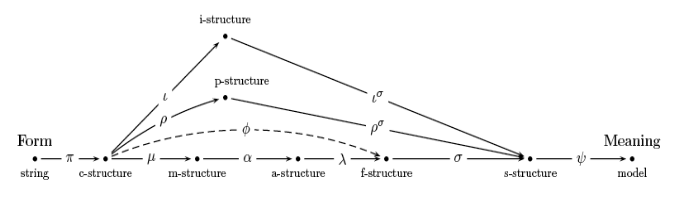
\includegraphics[scale=0.5]{upload/tex/figures/parallelprojection.png}
    \caption{This is the projection architecture}
    \label{fig-label1}
\end{figure}

Figure \ref{fig-label1} describes the projection architecture. 

\section{Linguistic exmaples}

You can refer to examples with \texttt{\\ref}. Like this \ref{ex:intro:ex1}.

\ex. \label{ex:intro:ex1} This is a simple linguistic example. 

\ex. Some text here 
\a. This is an example with subexamples
    \b. Second example


Here is an example with glossing.

\exg. The first line \\
    det first line \\
    \trans \textit{`The translation'}

\exg. The first line \\
    det {second first} line \\
    \trans \textit{`The translation'}

    This page explains linguistic examples: \url{https://ftp.tu-chemnitz.de/pub/tex/macros/latex/contrib/linguex/doc/linguex-doc.pdf}

    This sentence has a footnote.\footnote{This is a footnote.}

    \section{Tables}

    Go to \url{https://www.tablesgenerator.com/} to create tables:

    \begin{table}[]
    \centering
\begin{tabular}{l||ll}
a  & \multirow{3}{*}{b} & c  \\
1  &                    & 3  \\
ho &                    & ho
\end{tabular}
\caption{This is an example table}
\label{table:hohoho}
\end{table}

This is a reference to Table \ref{table:hohoho}

\section{Special symbols}

Use \url{https://detexify.kirelabs.org/classify.html} to find special symbols